\documentclass[a4paper]{extarticle}
\usepackage[utf8]{inputenc}
\usepackage[a4paper, margin=1in]{geometry}

\usepackage{amssymb}
\usepackage{amsmath}
\usepackage{enumitem}
\usepackage{tcolorbox}
\usepackage{fancyhdr}
\usepackage{graphicx}
\usepackage{float}

\setlength{\parindent}{0em}
\setlength{\parskip}{0.4em}

\definecolor{theoremblue}{RGB}{1, 73, 124}
\definecolor{corollaryblue}{RGB}{70, 143, 175}
\definecolor{exampleblue}{RGB}{137, 194, 217}

\newtcolorbox{tbox}{colback=theoremblue!20,colframe=theoremblue,
boxrule=0pt,arc=0pt,boxsep=2pt,left=2pt,right=2pt,leftrule=2pt}

\newtcolorbox{cbox}{colback=corollaryblue!20,colframe=corollaryblue,
boxrule=0pt,arc=0pt,boxsep=2pt,left=2pt,right=2pt,leftrule=2pt}

\newtcolorbox{ebox}{colback=exampleblue!20,colframe=exampleblue,
boxrule=0pt,arc=0pt,boxsep=2pt,left=2pt,right=2pt,leftrule=2pt}

\title{IntroML - Lecture Notes Week 8}
\author{Ruben Schenk, ruben.schenk@inf.ethz.ch}
\date{\today}

\pagestyle{fancy}
\fancyhf{}
\rhead{ruben.schenk@inf.ethz.ch}
\rfoot{Page \thepage}
\lhead{IntroML - Lecture Notes Week 8}

\begin{document}

\maketitle

\section{PyTorch Tutorial}

\textbf{Autodiff} is an automatic implementation in PyTorch which calculates the gradients automatically given the \textit{forward pass} (i.e. the chain of operations from input to output).

\begin{figure}[H]
    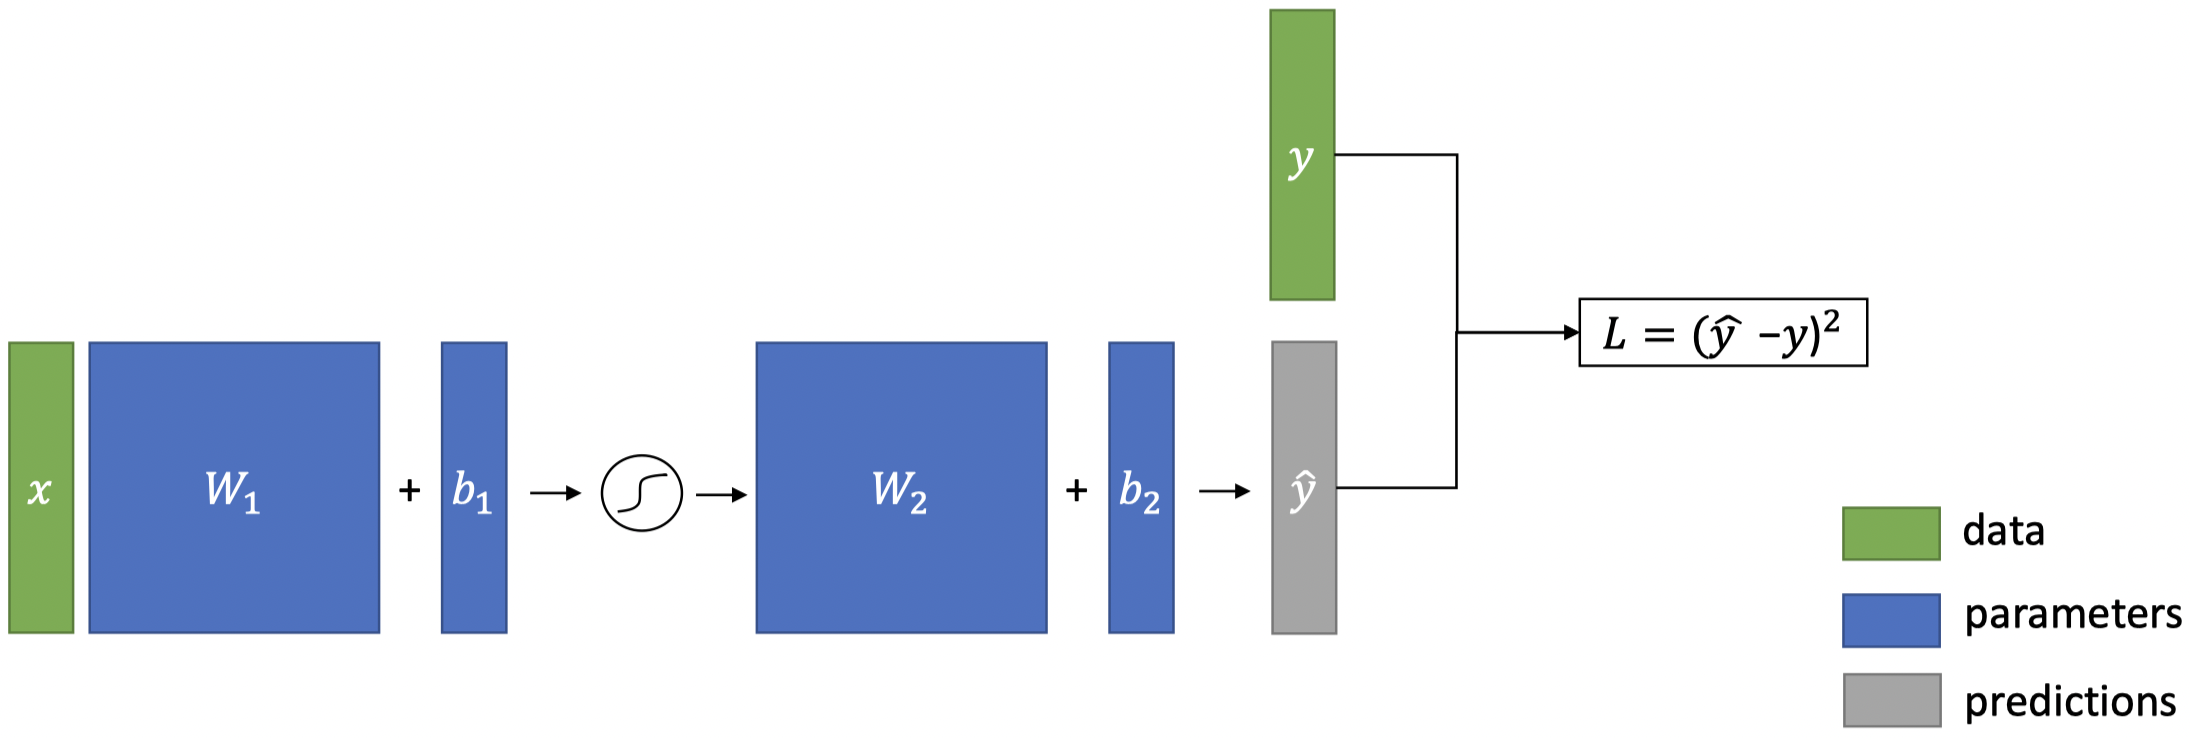
\includegraphics[width=15cm]{../images/IntroML_Fig8-1}
    \centering
\end{figure}

Given this forward pass, PyTorch automatically computes the derivatives (\textit{backward pass}) for us!

How does Autodiff work? First, as already mentioned, we need to provide the forward pass. Given that, PyTorch constructs the computation graph (DAG) and stores the intermediate computed values at each node of the graph.

Example: Consider the following simple function:
\begin{verbatim}
    def f(x, y):
        c = x + y
        d = c**2
        return x * d

    x = torch.tensor([3.0], requires_grad=True)
    y = torch.tensor([-1.0], requires_grad=True)
    f_val = f(x, y)
\end{verbatim}

For this function, we get the following forward pass:

\begin{figure}[H]
    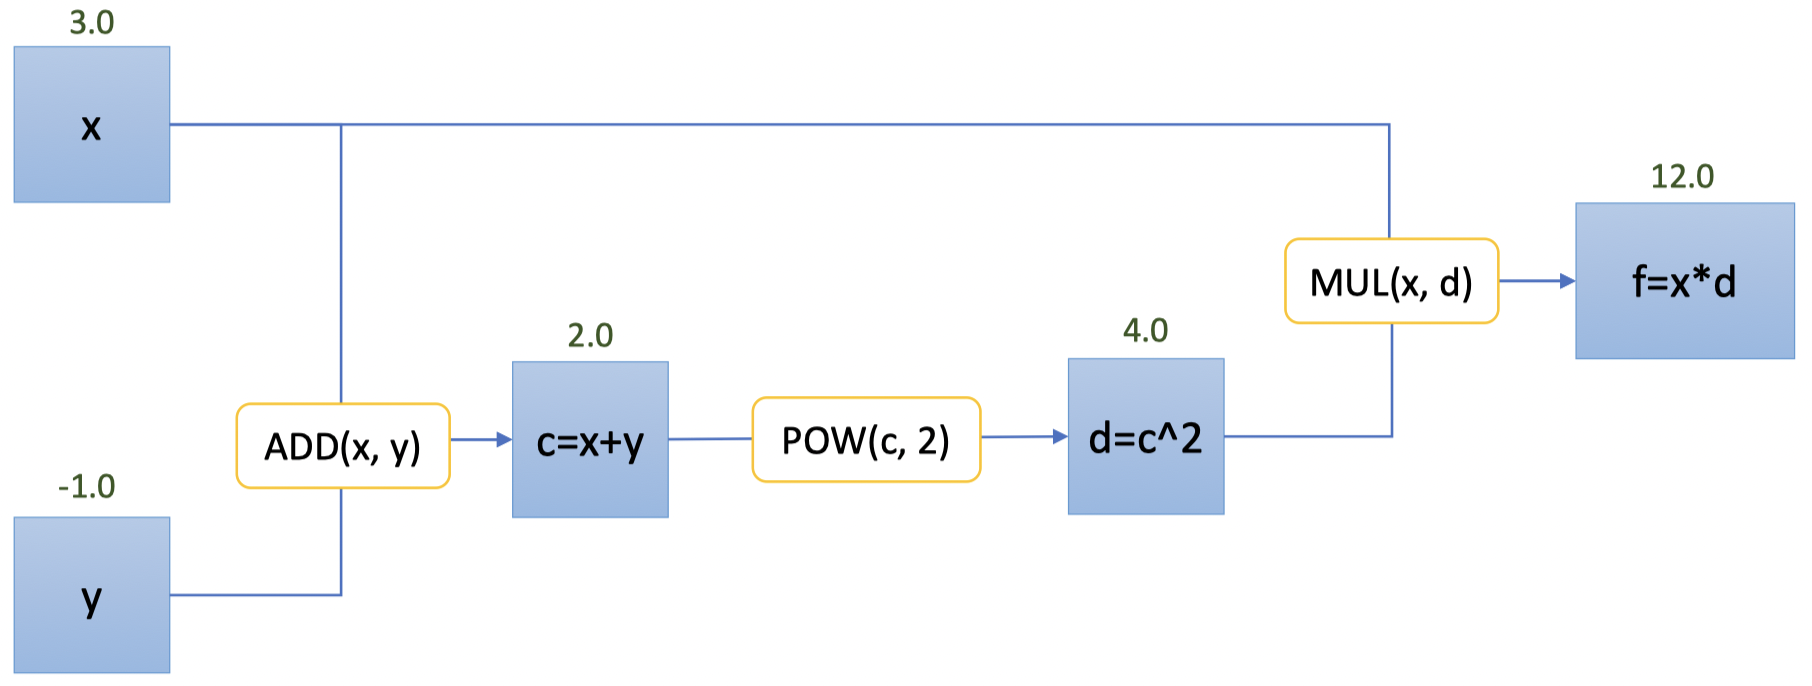
\includegraphics[width=15cm]{../images/IntroML_Fig8-2}
    \centering
\end{figure}

It is important to note here that every intermediate result is itself a tensor. Even if we override a variable, the previous tensor is kept alive.

Finally, Autodiff calculates the backward pass the following way:
\begin{itemize}
    \item Go back from the root (i.e. the loss) to the leaves (i.e. the parameters)
    \item Each elementary operation has a "backward function" that computes its derivatives
    \item We apply the chain rule along each path
    \item Total derivative is the sum of all path derivatives from the root to the leaf
\end{itemize}

\begin{figure}[H]
    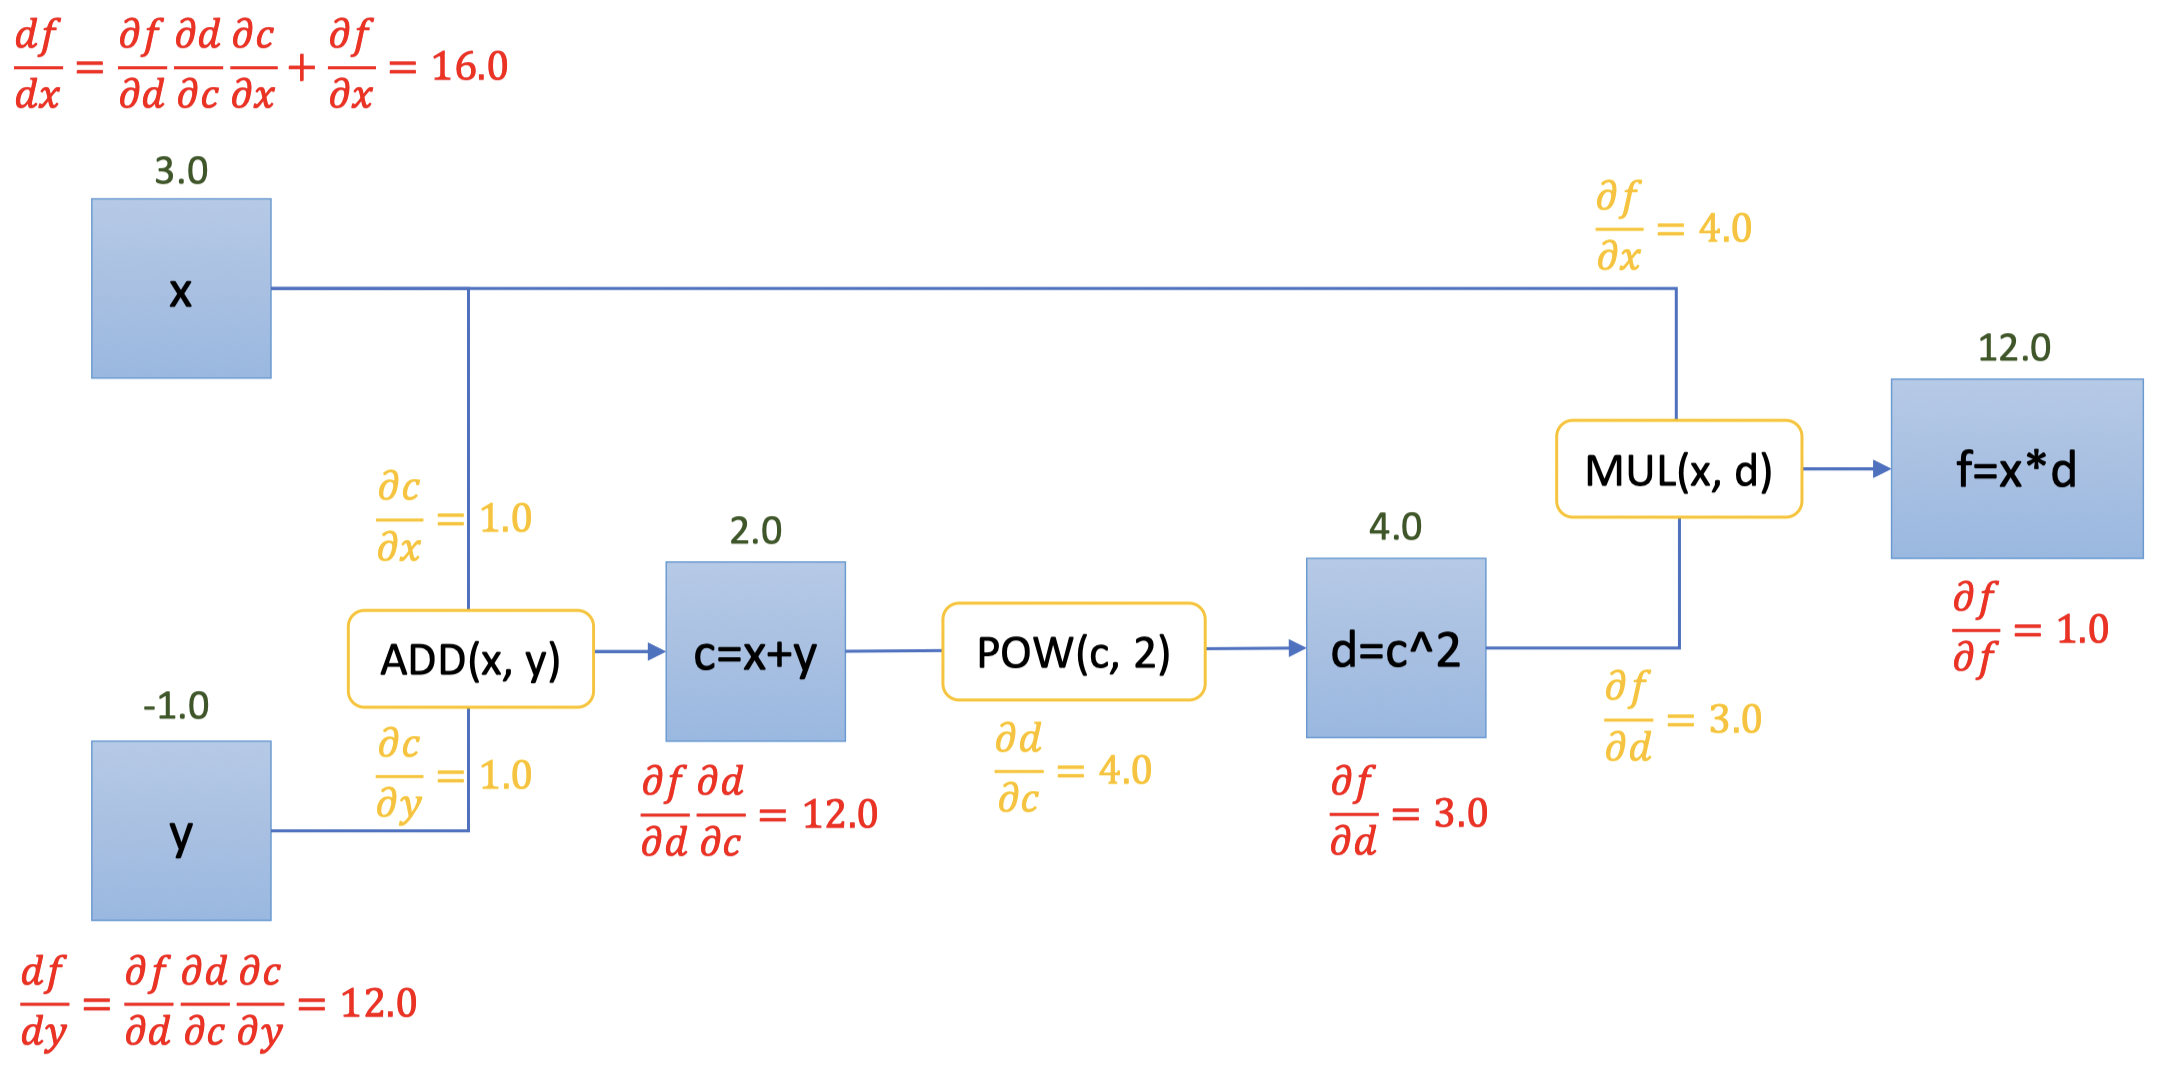
\includegraphics[width=15cm]{../images/IntroML_Fig8-3}
    \centering
\end{figure}

\section{Unsupervised Learning: Clustering}

\subsection{Introduction}

So far we have concerned ourselfes with \textit{supervised learning.} The idea behind that is that we have some dataset $X$ and their labels $Y$ from which we let the model learn the link between the data and the labels, such that it can label unlabelled data.

The idea behind \textbf{unsupervised learning} is that we only provide the dataset $X$ to the model (without the labels) and let the model learn the labels itself, based on some goals (e.g. grouping the data by similarities, understanding meaningful features, etc.).

What is \textbf{clustering?} The key idea behind clustering is, given some data points, to group them into clsuters such that:
\begin{itemize}
    \item \textit{Similar} points are in the same clsuter
    \item \textit{Dissimilar} points are in different clusters
\end{itemize}
Points are typically represented either in (high-dimensional) Euclidean space or with distances specified by a metric or (dis-)similarity function. Realted to this approach is \textit{anomal/outlier detection,} i.e. the identification of points that "don't fit well in any of the clusters".

There are some standard approaches to clustering:
\begin{itemize}
    \item \textit{Hierarchical clustering:} Build a tree (bottom-up or top-down), representing distances among data points. Examples: single-, average-linkage clustering
    \item \textit{Partitioning approaches:} Define and optimize a notion of "cost" defined over partitions. Examples: Spectral clustering, graph-cut based approaches
    \item \textit{Model-based approaches:} Maintain cluster "models" and infer cluster memebership (e.g. assign each point to closest center). Examples: k-means clustering, Gaussian mixture models, etc.
\end{itemize}

\subsection{k-Means Clustering}

The idea behind \textbf{k-means clustering} is as follows:
\begin{enumerate}
    \item Represent each cluster by a single point (center)
    \item Assing points to the closest center $\mu_i \in \mathbb{R}^d$
    \item Induces \textit{Voroni partition}
\end{enumerate}
Our data is given as $D = \{x_1,..., \, x_n\}, \, x_j \in \mathbb{R}^d$ and each $x_j$ is assigned a cluster $z_j = \arg \min_i ||x_j - \mu_i||_2, \, z_j \in {1,..., \, k}$.

\begin{figure}[H]
    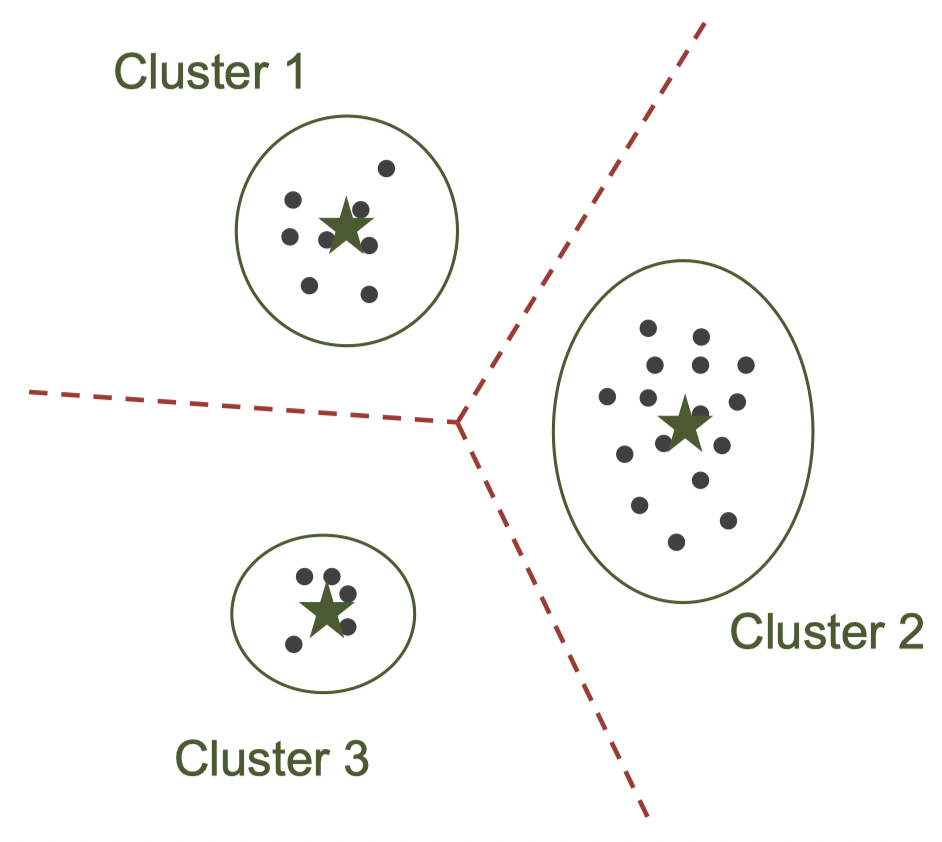
\includegraphics[width=8cm]{../images/IntroML_Fig8-4}
    \centering
\end{figure}

To reformulate, we may pose the k-means problem in the the following way:
\begin{itemize}
    \item Assume points are in Euclidean space $x_i \in \mathbb{R}^d$
    \item represent clusters as centers $\mu_j \in \mathbb{R}^d$
    \item Each point is assigned to the closest center
\end{itemize}
The goal is to pick centers to \textit{minimize the sum of squared distances,} i.e.
\[
    \text{minimize } \hat{R}(\mu) := \hat{R}(\mu_1,..., \, \mu_k) = \sum_{i = 1}^n \min_{j \in \{1,..., \, k\}} ||x_i - \mu_j||_2^2.
\]
In general this is a non-convex optimization and is NP-hard to solve!

\begin{cbox}
    \textbf{Algorithm (Lloyd's Heuristic):} The following represents on of the k-means algorithms:
    \begin{enumerate}
        \item Initialize cluster centers $\mu^{(0)} = [\mu^{(0)}_1,..., \, \mu^{(0)}_k]$
        \item While not converged:
        \begin{enumerate}
            \item Assign each point $x_i$ to the closest center
            \[
                z_i \leftarrow \arg \min_{j \in \{1,..., \, k\}} ||x_i - \mu^{(t-1)}_j||_2
            \]
            \item Update the center as the mean of assigned data points
            \[
                \mu^{(t)}_j \leftarrow \frac{1}{n_j} \sum_{i : z_i = j} x_i
            \]
        \end{enumerate}
    \end{enumerate}
\end{cbox}

K-means is \textit{guaranteed to monotonically decrease} the average squared distance in each iteration, i.e. $\hat{R}(\mu^t) \geq \hat{R}(\mu^{t + 1})$. In other words:
\begin{itemize}
    \item Given $\mu^t$, we obtain $z^z = \arg \min_z \hat{R}(\mu^t, \, z)$
    \item Given $z^t$, we obtain $\mu^t = \arg \min_{\mu}\hat{R}(\mu, \, z^t)$
\end{itemize}
From this, we have:
\[
    \hat{R}(\mu^t, \, z^t) \geq \hat{R}(\mu^{t + 1}, \, z^t) \geq \hat{R}(\mu^{t + 1}, \, z^{t + 1}).
\]
This converges to a \textit{local optimum} and the cost per iteration is $O(n \cdot k \cdot d)$.

However, k-means also poses some challenges:
\begin{itemize}
    \item Generally only converges to local optimum, the performance strongly depends on the initialization.
    \item Number of iterations required can be exponential. In practice however, the algorithm often converges quickly.
    \item Determining the number of clusters $k$ can be difficult.
    \item One cannot well model clusters of arbitrary shape.
\end{itemize}

\subsection{k-Means++ Clustering}

Lloyd's heuristic does not generally converge to the optimal solution since the performance depends heavily on the initialization.

One option for seeding would be \textit{random seeding,} though one can directly see some problems with this approach:

\begin{figure}[H]
    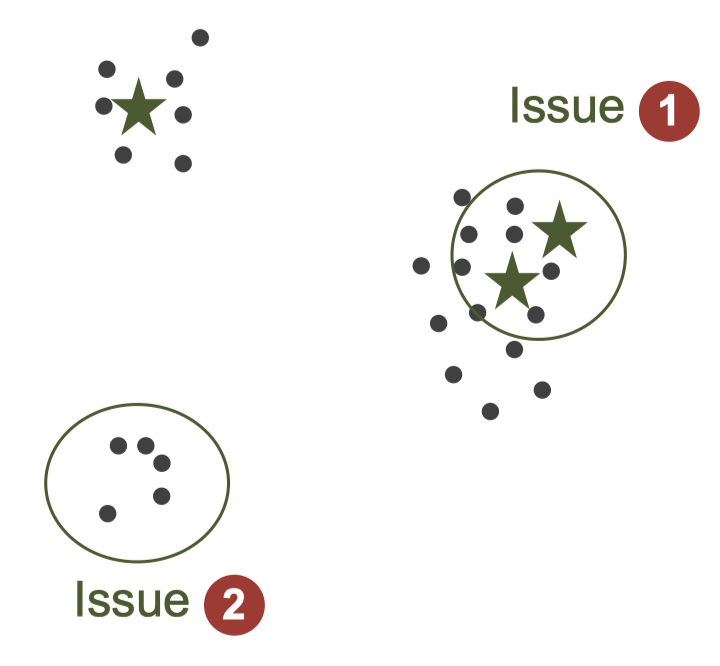
\includegraphics[width=8cm]{../images/IntroML_Fig8-5}
    \centering
\end{figure}

This is where the \textbf{k-means++} algorithm comes into play. It proposes adaptive seeding:

\begin{cbox}
    \textbf{Algorithm:} The k-means++ algorithm works in the following way:
    \begin{enumerate}
        \item Startwith a random point as the center
        \[
            \text{Prior } \mu_1^0 = x_1 \text{ where } i \sim Unif(1,..., \, n).
        \]
        \item Add centers $2...k$ randomly, proportionally to the squared distance to the closest selected center
        \[
            \text{Given } \mu_{1:j}^0 \text{ pick } \mu_{1:j+1}^0 = x_i \text{ where } p(i) = \frac{1}{z} \min_{l \in \{1,..., \, j\}}||x_i - \mu_l^0||_2^2
        \]
        \item We can show the the expected cost is $O(\log k)$ times that of the optimal k-means solution
        \[
            \text{Given } \hat{R}(\mu_{\text{k-means++}}) \leq O(\log k) \min_{\mu} \hat{R}(\mu)
        \]
    \end{enumerate}
\end{cbox}

\subsection{Model Selection}

In general, \textbf{model selection} (e.g. determining the number of clsuters) is difficult. There are several different approaches:
\begin{itemize}
    \item Heuristic quality measures
    \item Regularization, i.e. favoring simple models with few parameters by penalizing complex models
    \item Information theoretic basis (tradeoff between robustness (stability) and informativeness)
\end{itemize}

\begin{figure}[H]
    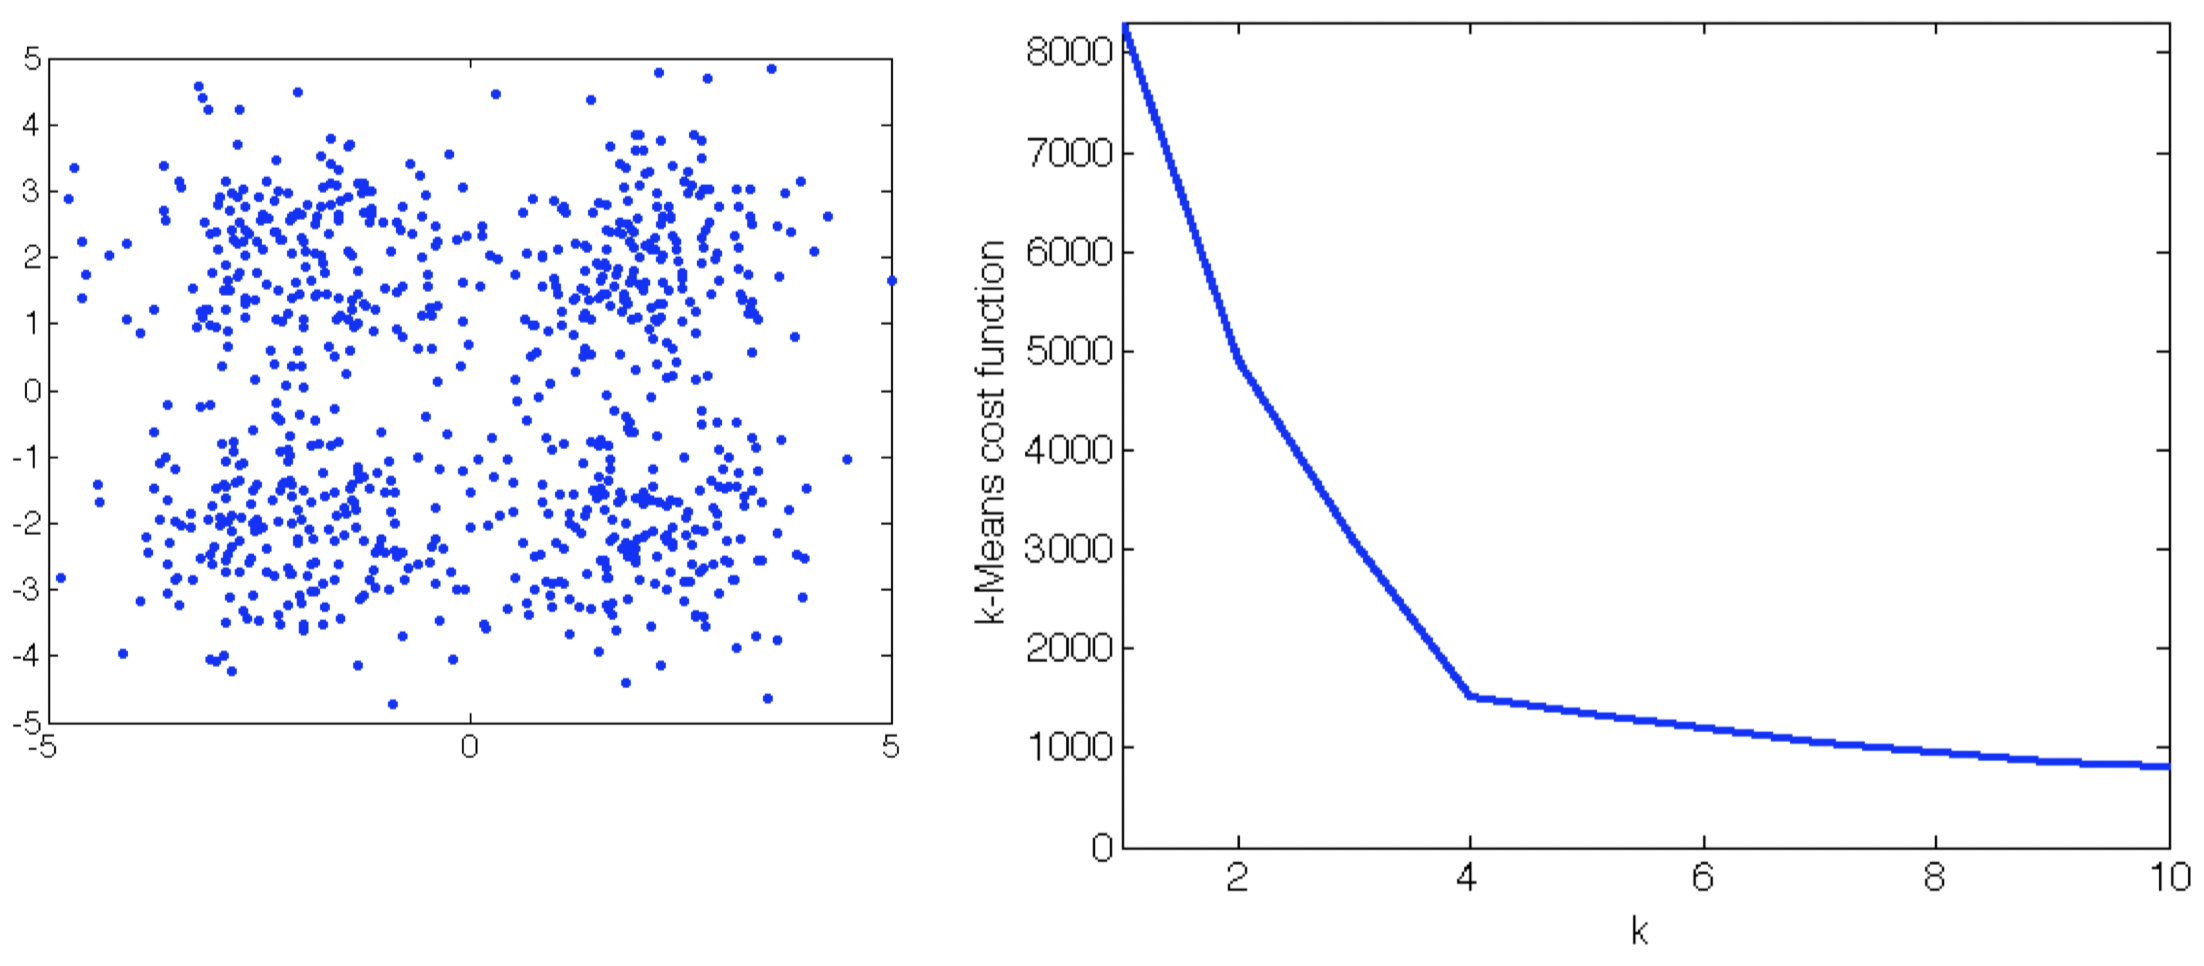
\includegraphics[width=15cm]{../images/IntroML_Fig8-6}
    \centering
\end{figure}

On \textbf{heuristic for determining} $k$ might be to find the $k$ that decreases our loss function. We then pick $k$ such that increasing $k$ leads to negligible decrease in loss.

Another idea is to use \textbf{regularization} and penalize models with higher $k$, i.e.:
\[
    \min_{k, \, \mu_{1:k}} \hat{R}(\mu_{1:k}) + \lambda \cdot k.
\]

\begin{figure}[H]
    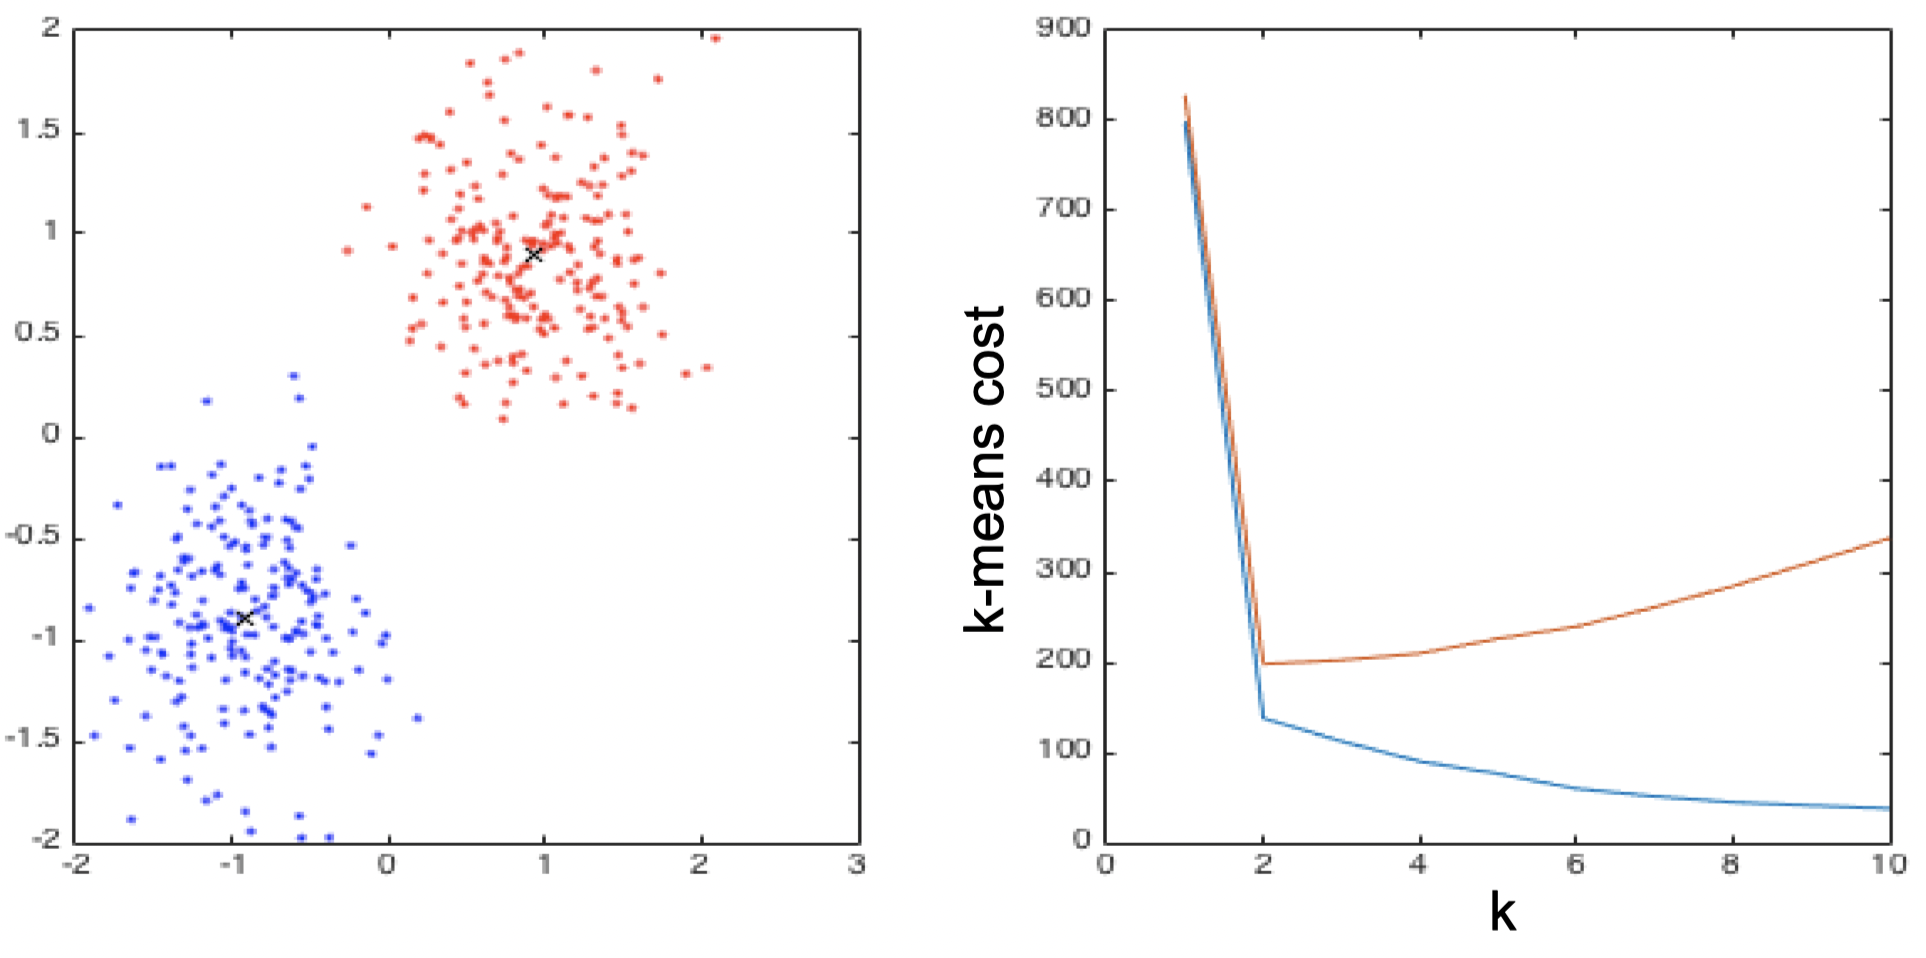
\includegraphics[width=15cm]{../images/IntroML_Fig8-7}
    \centering
\end{figure}

This approach poses another problem since we now have to choose a "correct" $\lambda$, however, this is usually easier than choosing the "correct" $k$.

\subsection{Challenges with k-Means}

To summarize, we again list some of the challenges encountered when working with k-means:
\begin{enumerate}
    \item Generally only converges to local optimum
    \item Number of iterations required can be exponential
    \item Cannot well model clusters of arbitrary shape
    \item Determining the number of clusters $k$ is difficult
\end{enumerate}

Problem 1 and 2 are practically not a big issue. Problem 3 can be fixed via kernel-k-means which we'll introduce later. Problem 4 is unsolved and also a practical problem.

\end{document}